\documentclass[10pt]{beamer}

\usepackage[utf8]{inputenc}
 
 
%Information to be included in the title page:
\title{CU01. Crear Sucursal}
\subtitle{Módulo: Sucursal}
\author{Edgar Felipe Fuentes Perea}
\institute{Softtek}
\date{2018}
\logo{
\includegraphics[height=0.5cm]{img/Softtek_1ink_SMALL.jpg}}
\usetheme{Copenhagen}
%\usefonttheme{structuresmallcapsserif}
\usepackage{bookman}

\newcounter{rtaskno}
\newcommand{\rtask}{%
   \stepcounter{rtaskno}%
   \thertaskno}

\begin{document}
 
\frame{\titlepage}
 
\begin{frame}
	\frametitle{Disparador}
	Administrador solicita la página \textit{[Crear Sucursal]}.
\end{frame}

\begin{frame}
	\frametitle{Escenario Principal}
	\rtask. El Sistema muestra la página \textit{[Crear Sucursal]}.\\
	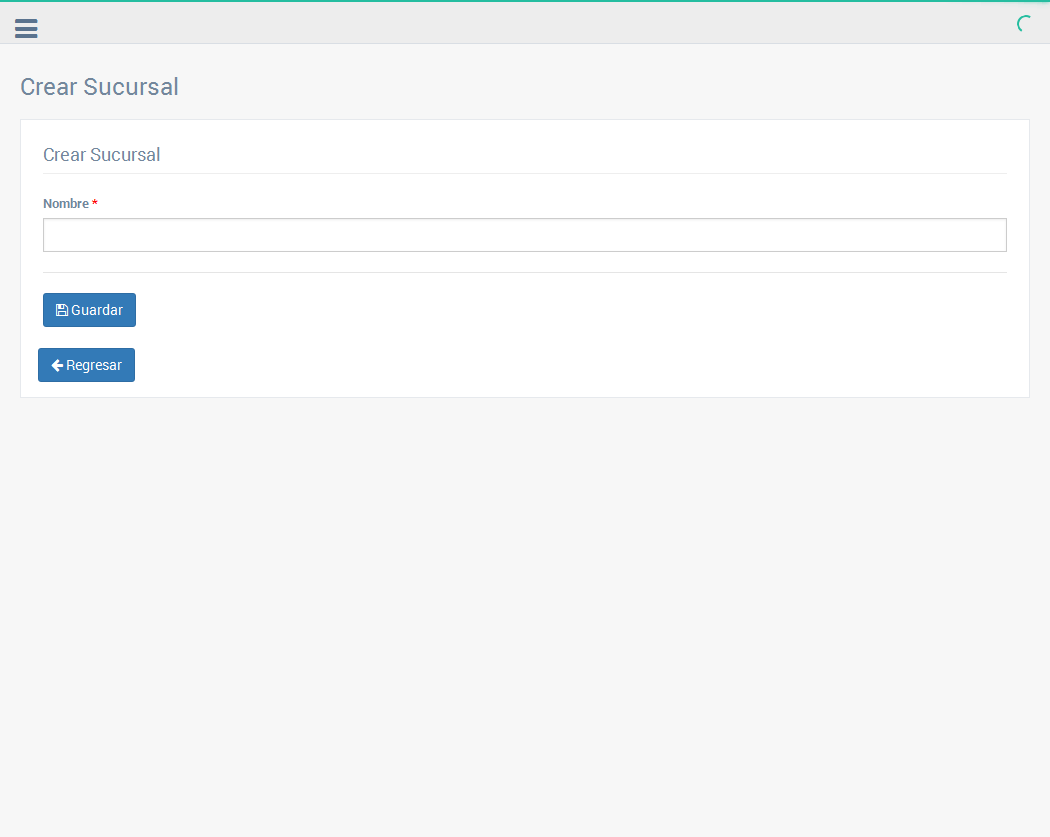
\includegraphics[width=\linewidth]{screenshoots/sucursalservices/crearsucursal-main/step-03.png}
\end{frame}
 
\begin{frame}
	\frametitle{Escenario Principal}
	\rtask. Administrador captura información en la forma \textit{[Crear Sucursal]}.\\
	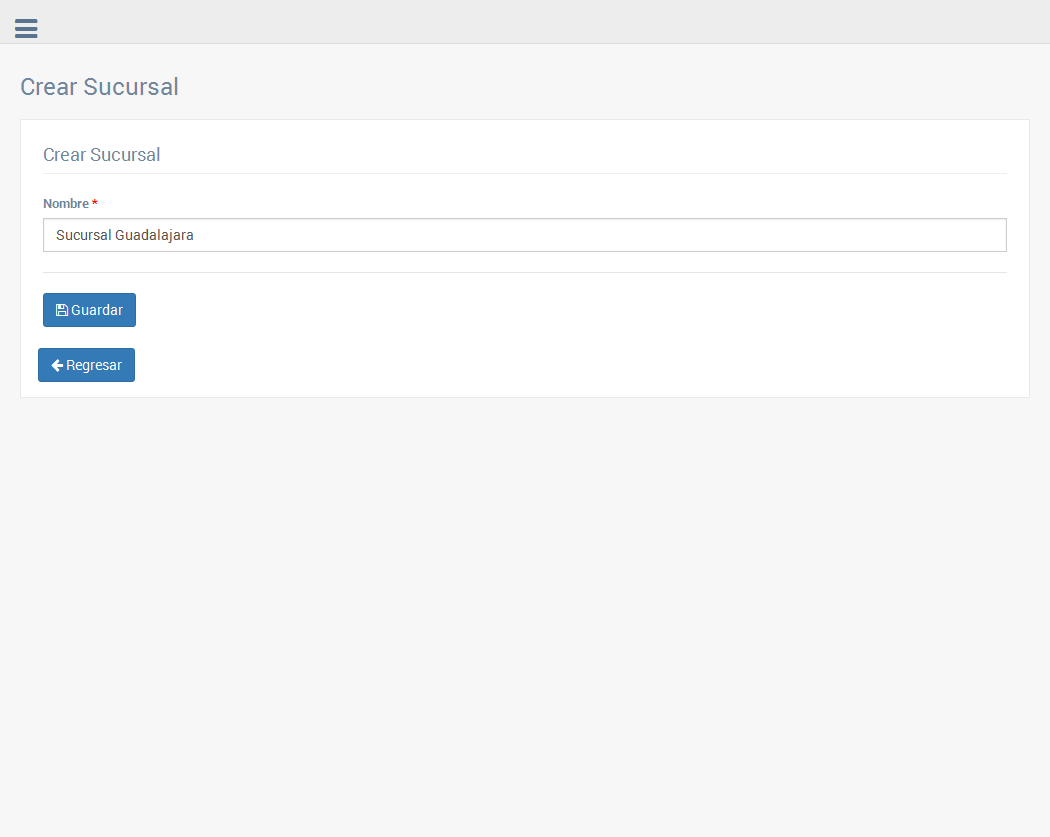
\includegraphics[width=\linewidth]{screenshoots/sucursalservices/crearsucursal-main/step-04.png}
\end{frame}

\begin{frame}
	\frametitle{Escenario Principal}
	\rtask. Administrador elige el comando \textit{[Guardar]}.\\
	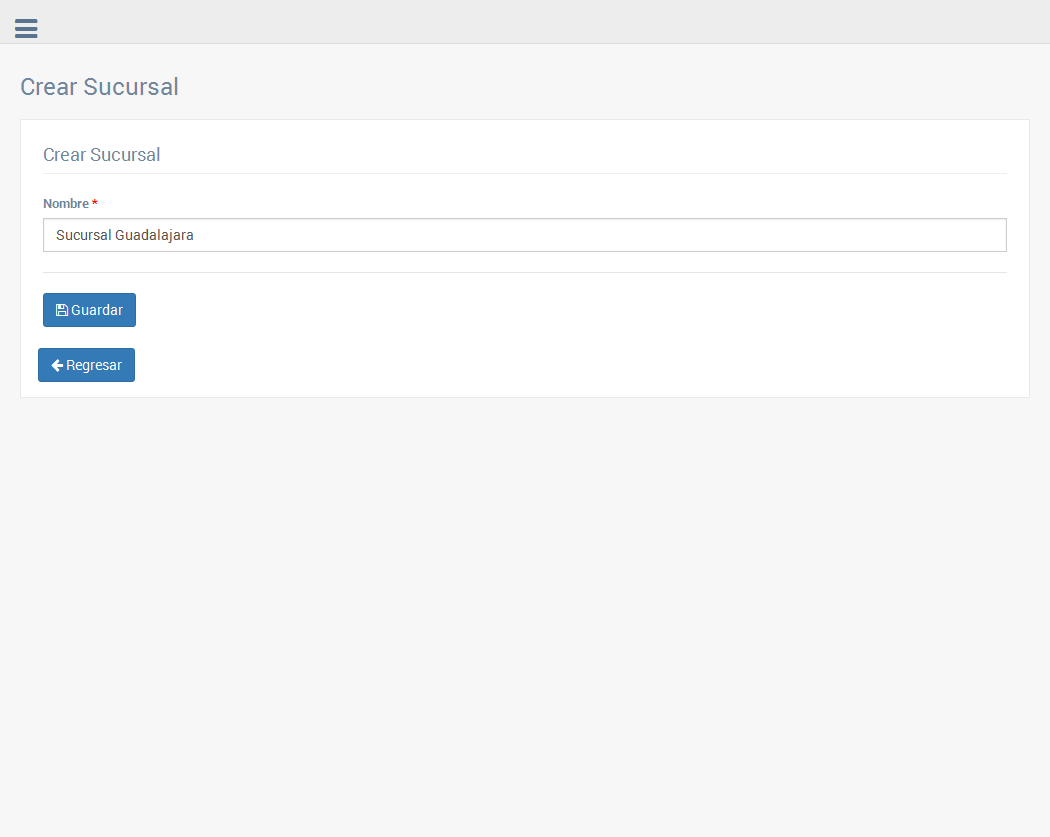
\includegraphics[width=\linewidth]{screenshoots/sucursalservices/crearsucursal-main/step-04.png}
\end{frame}

\begin{frame}
	\frametitle{Escenario Principal}
	\rtask. El Sistema valida que los datos de la forma \textit{[Crear Sucursal]} estan completos.\\
	\hyperlink{ex01}{\beamergotobutton{Excepción: Datos incompletos}}
	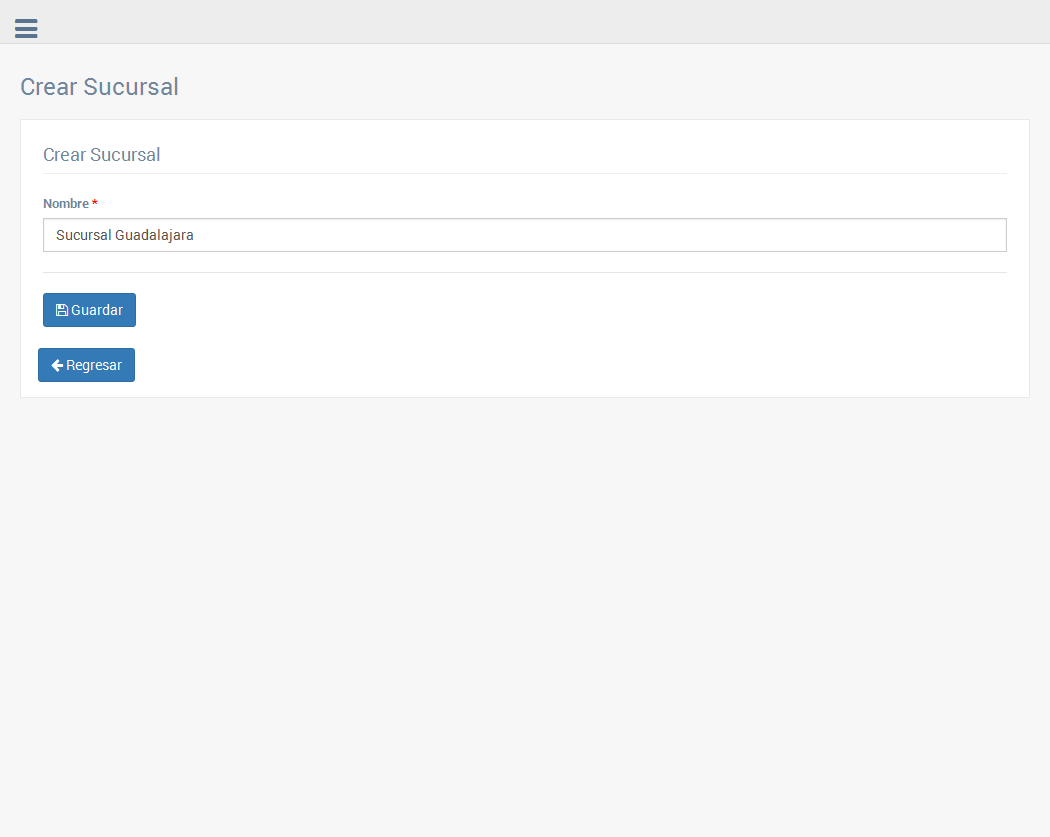
\includegraphics[width=\linewidth]{screenshoots/sucursalservices/crearsucursal-main/step-04.png}
\end{frame}

\begin{frame}
	\frametitle{Escenario Principal}
	\rtask. El Sistema crea un nuevo registro en la entidad \textit{[Sucursal]}.\\
	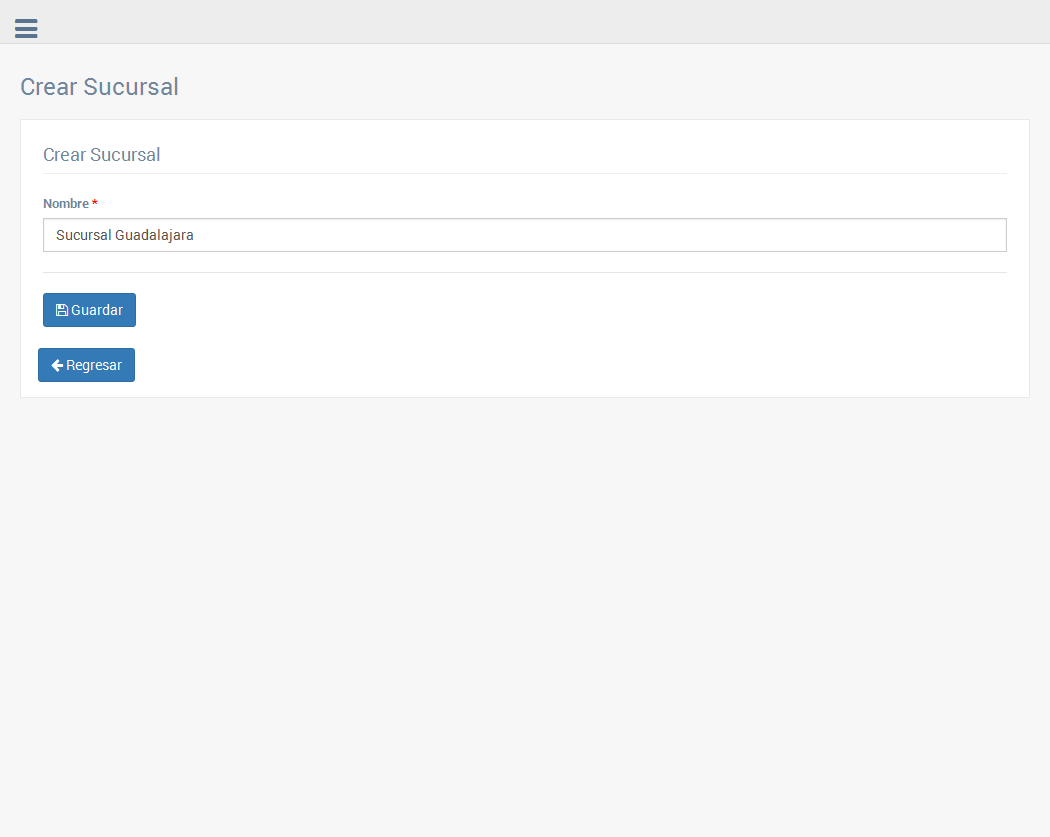
\includegraphics[width=\linewidth]{screenshoots/sucursalservices/crearsucursal-main/step-04.png}
\end{frame}

\begin{frame}
	\frametitle{Escenario Principal}
	\rtask. El Sistema muestra la página \textit{[Buscar Sucursal]}.\\
	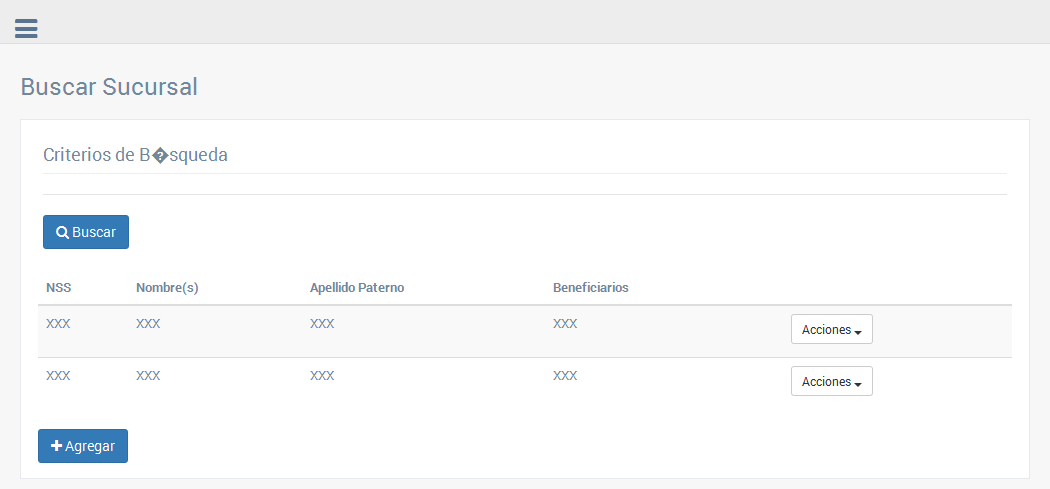
\includegraphics[width=\linewidth]{screenshoots/sucursalservices/crearsucursal-main/step-05.png}
\end{frame}

\begin{frame}
	\frametitle{Escenario Principal}
	\rtask. Fin del Caso de Uso.
\end{frame}

\begin{frame}
	\frametitle{Excepción: Datos incompletos }
	\hypertarget{ex01}{El Sistema muestra los campos que son requeridos.}\\
	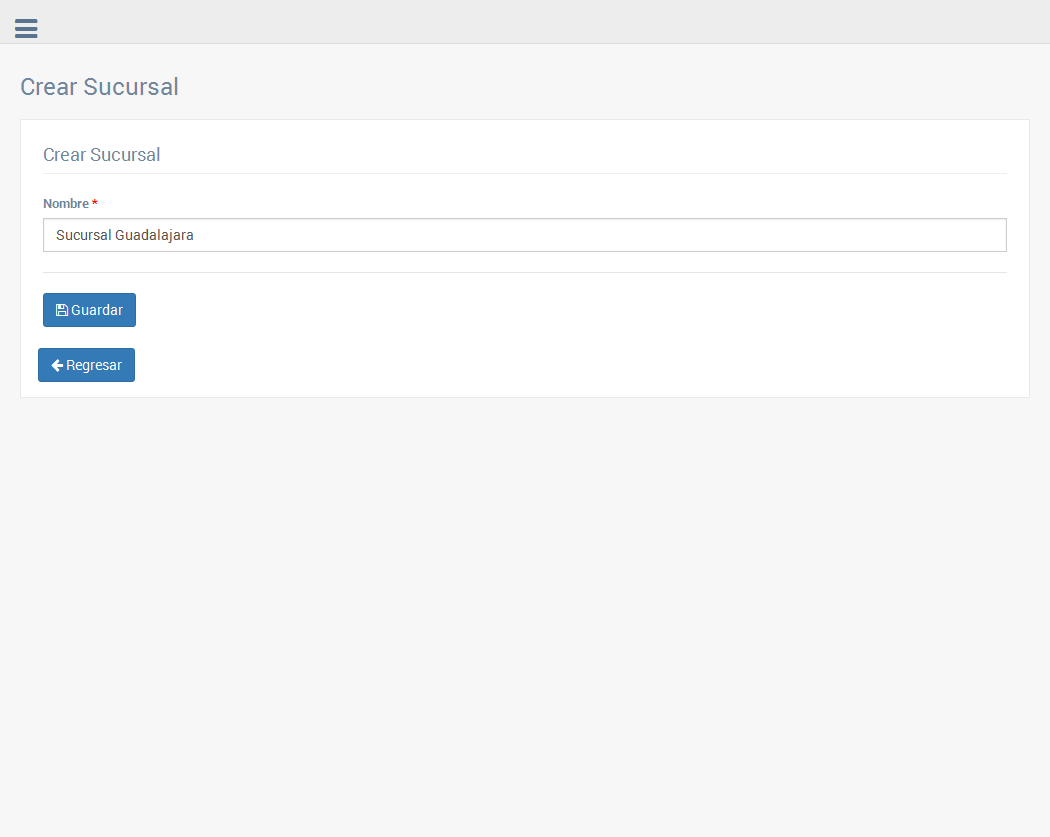
\includegraphics[width=\linewidth]{screenshoots/sucursalservices/crearsucursal-main/step-04.png}
\end{frame}

\end{document}